\documentclass[12pt]{article}


\usepackage{amssymb}
\usepackage{amsmath}
\usepackage{fullpage}
\usepackage{epsfig}
\usepackage{epstopdf}
\everymath{\displaystyle}



\begin{document}

\begin{center}
\underline{\LARGE{Chapter 3.4 Practice Problems}}
\end{center}

\noindent EXPECTED SKILLS:

\begin{itemize}

\item Be able to solve related rates problems. It may be helpful to remember the following strategy:

\begin{enumerate}

\item Read the problem carefully.

\item Draw a diagram, if possible, representing the situation at an arbitrary time $t$.

\item Introduce notation, making sure to assign symbols to all quantities which are functions of time.

\item Express the given information and the rate that you are trying to find in terms of derivatives.

\item Write an equation which relates the various quantities of the problem. 

\item Differentiate both sides with respect to $t$.  (Keep in mind which quantites are functions of $t$ and which quantities are remaining constant.)

\item Substitute all of the relevant information into the resulting equation and solve for the the unknown rate.

\end{enumerate}

\end{itemize}

\noindent PRACTICE PROBLEMS:

\medskip

\begin{enumerate}

\item Assume that $x=x(t)$ and $y=y(t)$.  Use the given information to find the indicated rate of change.

\begin{enumerate}

\item Suppose $y=3x^5-7$ and $\frac{dx}{dt}=4$ when $x=2$.  Compute $\frac{dy}{dt}$ when $x=2$.

\includegraphics[scale=0.5]{start.pdf}
{{$960$}}
\includegraphics[scale=0.5]{end.pdf}


\item Suppose $x^2+2xy+y^3=4$ and $\frac{dx}{dt}=-4$ at the point $(-3,1)$.  Compute $\frac{dy}{dt}$ at $(-3,1)$.

\includegraphics[scale=0.5]{start.pdf}
{{$\frac{16}{3}$}}
\includegraphics[scale=0.5]{end.pdf}


\end{enumerate}

\item A point is moving on the graph of $xy=24$.  At the moment when $y=3$, the $y$ coordinate is increasing at a rate of $2$ units per second.  How fast is the $x$ coordinate changing at that moment?

\includegraphics[scale=0.5]{start.pdf}
{{$-\frac{16}{3}$ units per second}}
\includegraphics[scale=0.5]{end.pdf}


\item A boat is being pulled towards a dock by a rope.  The rope is attached to the bow of the boat and is pulled through a pulley which is 4 feet above the dock, as shown in the sketch below.  If the rope is being pulled in at a constant rate of 2 feet per second, how fast is the distance between the boat and the dock changing at the instant when the boat is 10 feet from the dock?

\begin{center}
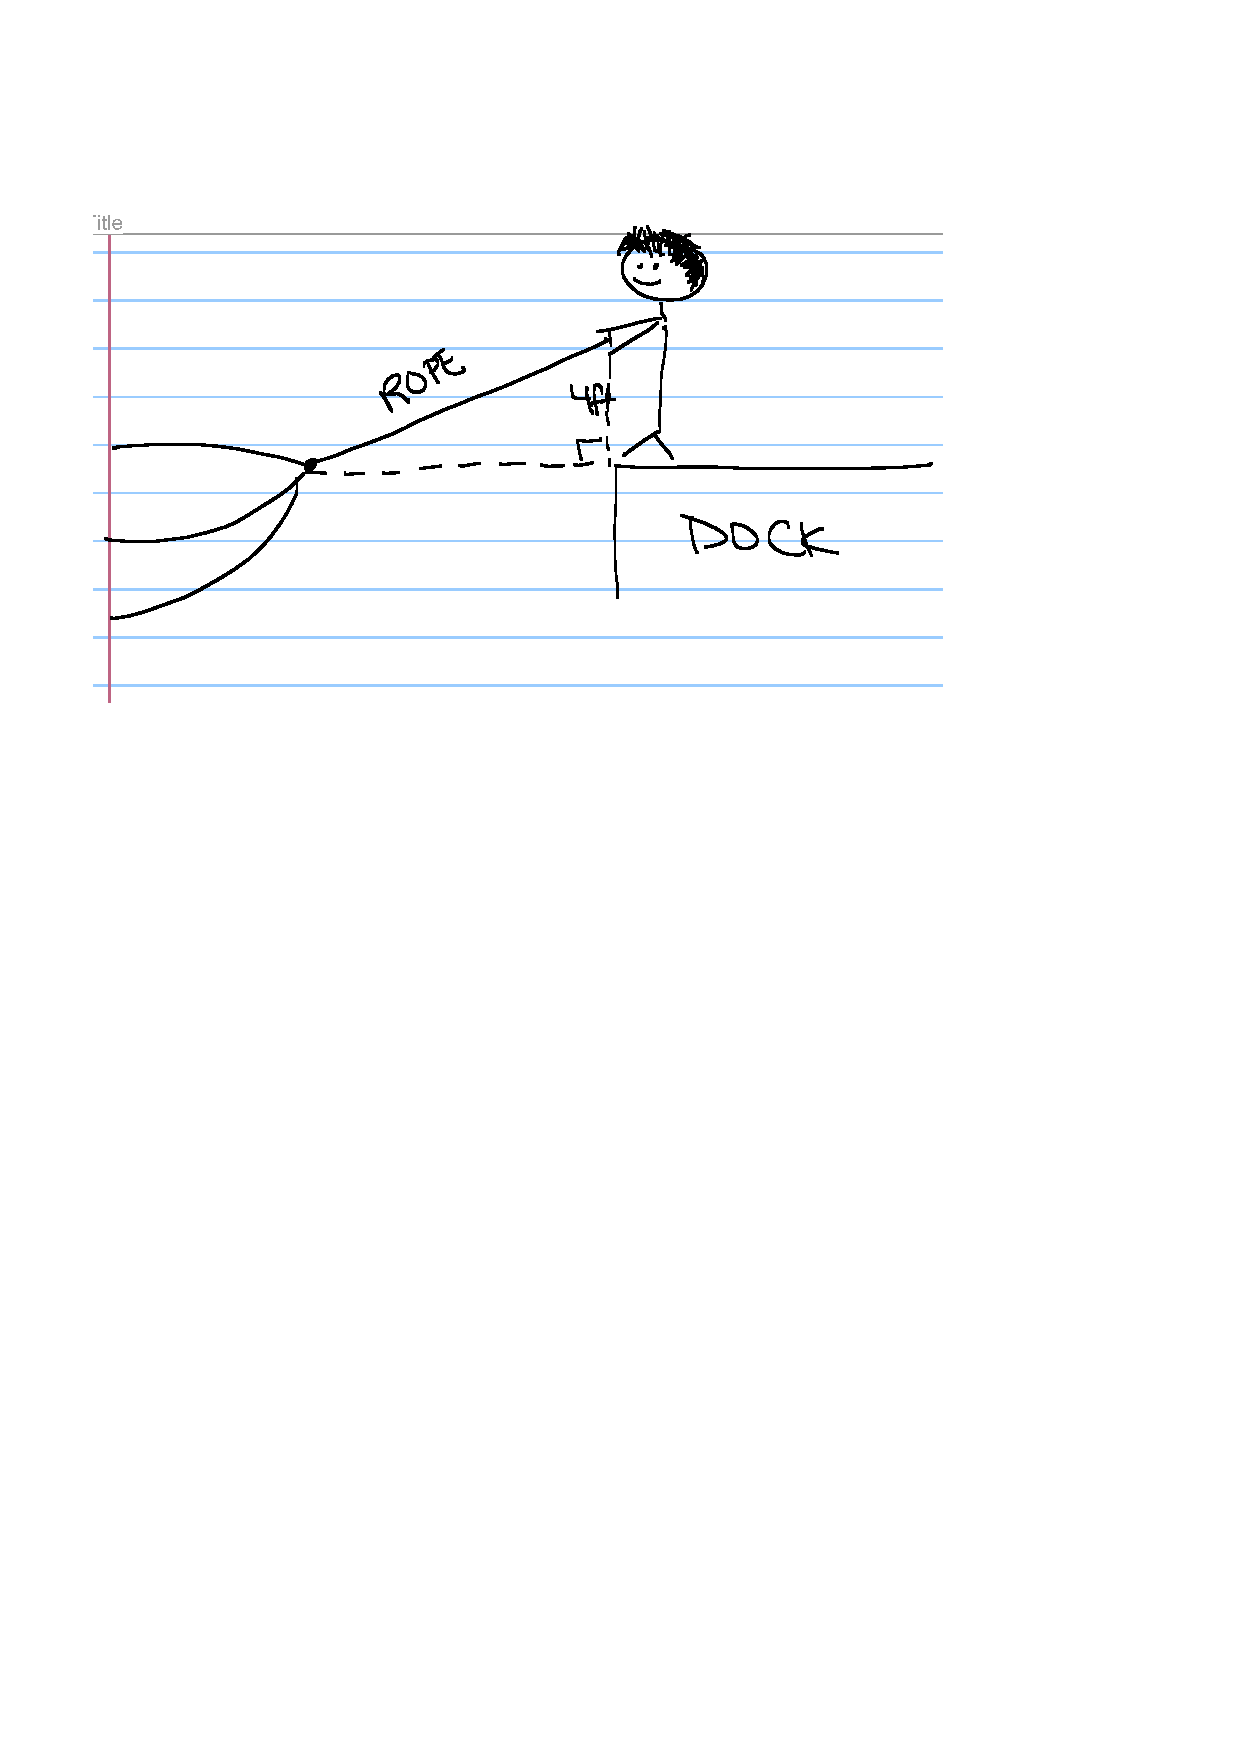
\includegraphics[scale=0.5]{boat.pdf}
\end{center}

\includegraphics[scale=0.5]{start.pdf}
{{$-\frac{\sqrt{116}}{5}$ feet per second}}
\includegraphics[scale=0.5]{end.pdf}


\item A plane flying horizontally at an altitude of 2 miles and a constant speed of 1000 miles per hour passes directly over a radar station.  At the instant when it is 4 miles away from the station, how fast is the plane's distance from the station increasing?

\includegraphics[scale=0.5]{start.pdf}
{{$500\sqrt{3}$ miles per hour}}
\includegraphics[scale=0.5]{end.pdf}


\item Two cars start moving from the same point.  Car A travels due south at 20 miles per hour and car B travels due west at 15 miles per hour.  At what rate is the distance between cars A and B increasing after 2 hours?

\includegraphics[scale=0.5]{start.pdf}
{{25 miles per hour}}
\includegraphics[scale=0.5]{end.pdf}


\item A 24 foot plank is leaning against a vertical wall.  The bottom of the plank is pushed towards the wall at a constant rate of 3 ft/min.  How fast is the acute angle that the plank makes with the ground changing at the instant when the bottom of the plank is 12 ft from the wall?  Your answer should include the appropriate units.

\includegraphics[scale=0.5]{start.pdf}
{{$\frac{1}{4\sqrt{3}}$ radians per minute}}
\includegraphics[scale=0.5]{end.pdf}


\item The blood that Dexter drips from his dropper onto a slide spreads in a circle whose area increases at a constant rate of 2 square millimeters per second.  How fast is the radius of the drop increasing at the instant when the area is 6 square millimeters? 

\includegraphics[scale=0.5]{start.pdf}
{{$\frac{1}{\sqrt{6\pi}}$ millimeters per second}}
\includegraphics[scale=0.5]{end.pdf}


\item A spherical snowball melts in such a way that its surface area decreases at a constant rate of 2 square centimeters per minute.  Find the rate at which the radius is changing at the instant when the diameter is $\frac{1}{2}$ centimeter?

\includegraphics[scale=0.5]{start.pdf}
{{$-\frac{1}{\pi}$ cm per min}}
\includegraphics[scale=0.5]{end.pdf}


\item Recall that the volume $V$ of a right circular cylinder of radius $r$ and height $h$ (as shown below) is $V=\pi r^2h$.

\begin{center}
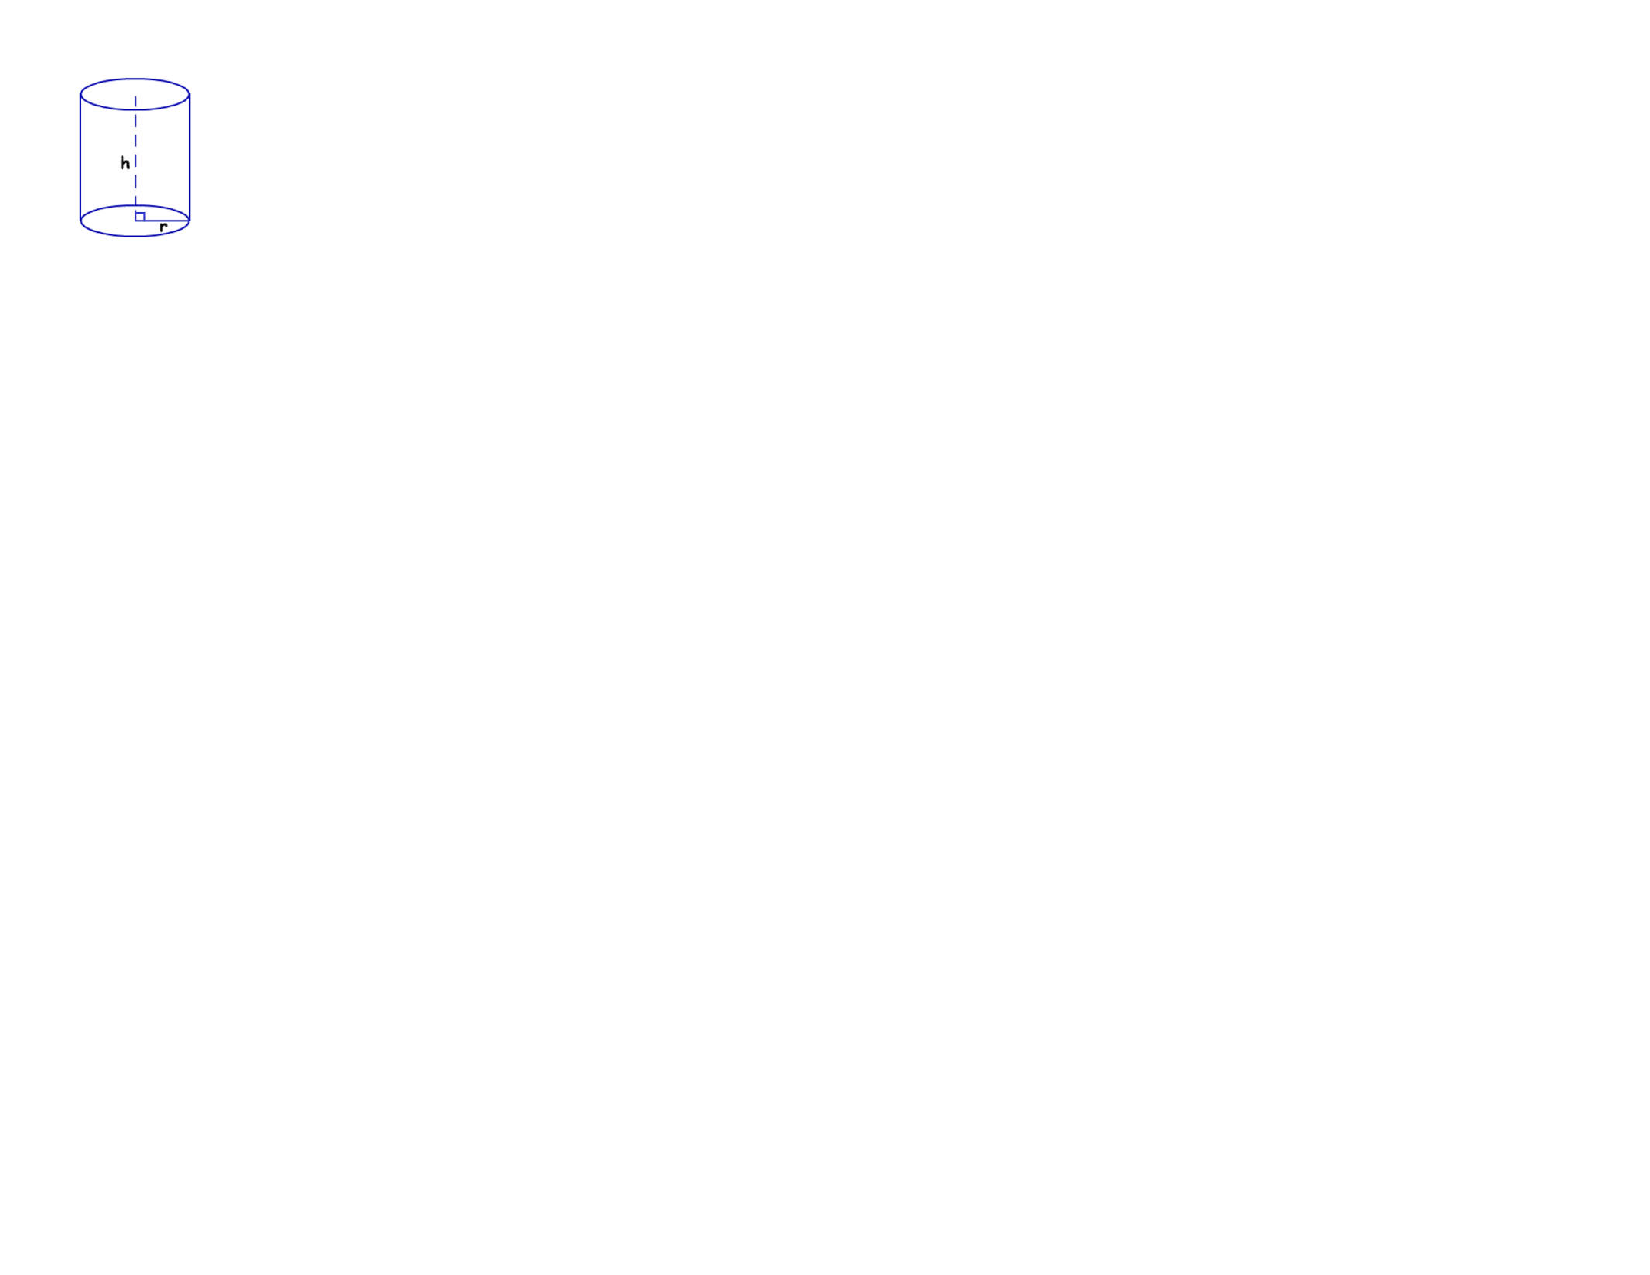
\includegraphics[scale=1]{cylinder.pdf}
\end{center}

\begin{enumerate}

\item How is $\frac{dV}{dt}$ related to $\frac{dr}{dt}$ if $h$ is constant and $r$ varies with time?

\includegraphics[scale=0.5]{start.pdf}
{{$\frac{dV}{dt}=2\pi r h \frac{dr}{dt}$}}
\includegraphics[scale=0.5]{end.pdf}


\item How is $\frac{dV}{dt}$ related to $\frac{dh}{dt}$ if $r$ is constant and $h$ varies with time?

\includegraphics[scale=0.5]{start.pdf}
{{$\frac{dV}{dt}=\pi r^2 \frac{dh}{dt}$}}
\includegraphics[scale=0.5]{end.pdf}


\item How is $\frac{dV}{dt}$ related to $\frac{dr}{dt}$ and $\frac{dh}{dt}$ if both $h$ and $r$ vary with time?

\includegraphics[scale=0.5]{start.pdf}
{{$\frac{dV}{dt}=\pi\left(r^2 \frac{dh}{dt}+2rh \frac{dr}{dt}\right)$}}
\includegraphics[scale=0.5]{end.pdf}


\end{enumerate}

\item Sand falling from a chute at a rate of 8 cubic feet per minute forms a conical pile whose height is always 3 times its radius.  How fast is the radius increasing at the instant when the height of the pile is 12 feet? 

\includegraphics[scale=0.5]{start.pdf}
{{$\frac{1}{6\pi}$ ft per min}}
\includegraphics[scale=0.5]{end.pdf}


\newpage

\item The trough pictured below is 15 feet long and 4 feet wide at the top.  The ends of the trough are isosceles triangles with a height of 3 feet.  If the water runs into the trough at the rate of 4 cubic feet per second, how fast is the water level rising at the instant when the water is 2 feet deep? (Recall: The volume of such a trough is $V=\frac{1}{2}lwh$)
\begin{center}
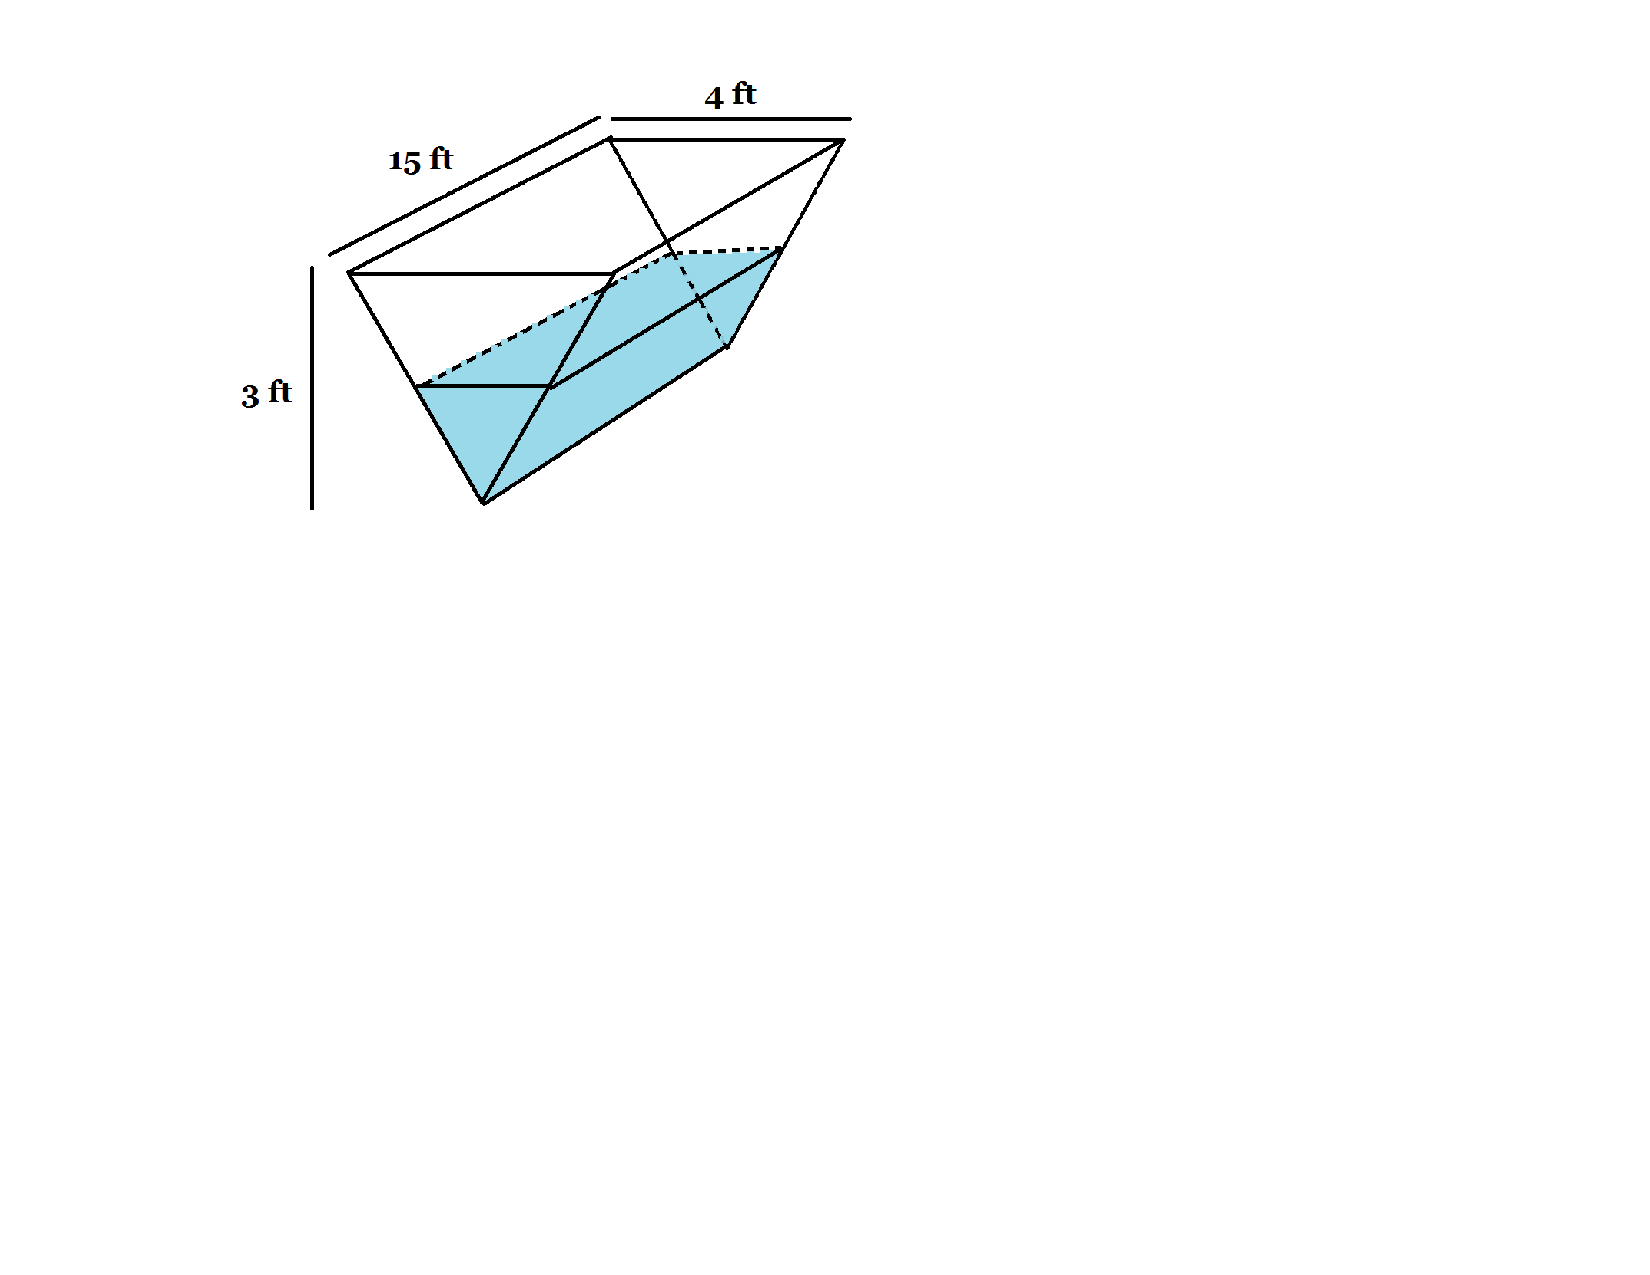
\includegraphics[scale=0.6]{trough.pdf}
\end{center}
\includegraphics[scale=0.5]{start.pdf}
{{$\frac{1}{10}$ feet per second}}
\includegraphics[scale=0.5]{end.pdf}


\item {\bf Multiple Choice:} Consider the triangle shown below.
\begin{center}
\setlength{\unitlength}{.4in}
\begin{picture}(7,5)(0,0)
\linethickness{1pt}
\put(0,0){\line(1,0){4}}
\put(4,0){\line(0,1){3}}
\put(0,0){\line(4,3){4}}
%\put(2,-.25){\makebox(0,0){$4$}}
\put(4.25,1.5){\makebox(0,0){$x$}}
\put(2,2){\makebox(0,0){$5$}}
\put(0.7,0.2){\makebox(0,0){$\theta$}}
\end{picture}
\end{center}
If $\theta$ increases at a constant rate of 3 radians per minute, at what rate is $x$ increasing in units per minute at the instant when $x$ equals 3 units?

\begin{enumerate}

\item 3

\item $\frac{15}{4}$

\item 4

\item 9

\item 12

\end{enumerate}

\includegraphics[scale=0.5]{start.pdf}
{{E}}
\includegraphics[scale=0.5]{end.pdf}


\item Two sides of a triangle have fixed lengths of 12 feet and 15 feet, respectively, and the angle between them is increasing at a rate of $2$ radians per minute.  How fast is the length of the third side increasing when the angle between the sides of fixed length is $\frac{\pi}{3}$ radians?  Hint: Consider the law of cosines.

\includegraphics[scale=0.5]{start.pdf}
{{$\frac{60}{\sqrt{7}}$ feet per minute}}
\includegraphics[scale=0.5]{end.pdf}


\item A street light is mounted at the top of a 19 foot-tall pole.  A 6 foot tall man walks away from the pole at a speed of 5 feet per second along a straight path.  How fast is the length of his shadow changing at the instant when he is 24 feet from the pole?

\includegraphics[scale=0.5]{start.pdf}
{{$\frac{30}{13}$ feet per second}}
\includegraphics[scale=0.5]{end.pdf}


\item A lighthouse is located on a small island $2$ km away from the nearest point $P$ on a straight shoreline.  If the light makes 3 revolutions per minute (counterclockwise), how fast is the beam of light moving along the shoreline at the instant when it is 1 km from $P$?

\includegraphics[scale=0.5]{start.pdf}
{{$15\pi$ km per minute}}
\includegraphics[scale=0.5]{end.pdf}


\end{enumerate}

\end{document}